
\begin{problem}{RNNs and LSTMs \hfill [40 pts]}{prob:rnns}
\label{prob:rnns}

Recurrent Neural Networks (RNNs) were one of the first models aimed at handling sequential data. In this set we will focus on Simple RNNs, also called Elman Networks. Below is a figure of a Simple RNN.

\begin{center}
    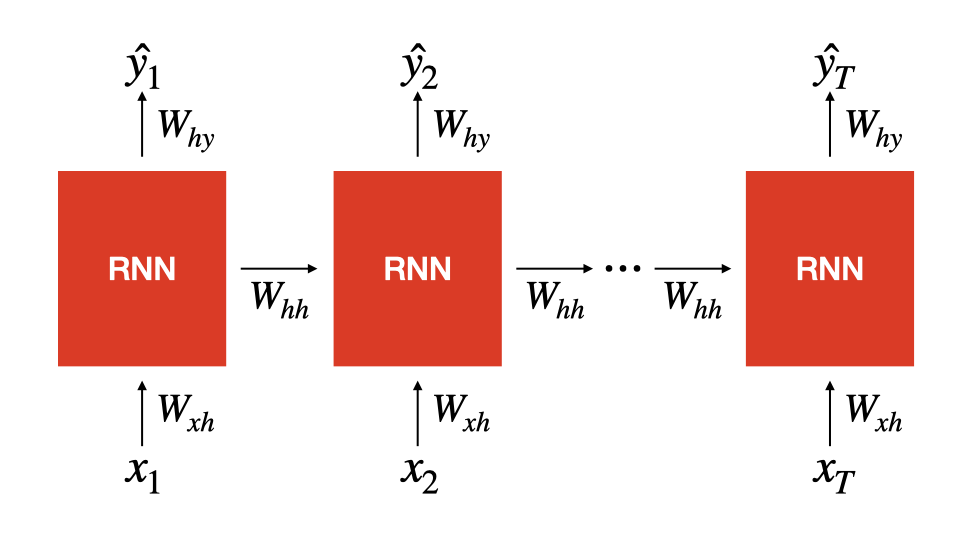
\includegraphics[width=0.75\linewidth]{media/rnnfig2.001.png}
\end{center}
    
The hidden state and output state computations are
$$h_t=\sigma(W_{hh}h_{t-1} + W_{xh}x_t + b_h)$$
$$\hat{y}_t = W_{hy}h_t + b_y$$

for $t = 1, \dots, T$. Note that the loss is $$\mathcal{L} = \sum_{t = 1}^T\mathcal{L}_t(y_t, \hat{y_t})$$

where $\mathcal{L}_t$ is the same for all timesteps.
\\
\\
\begin{adjustwidth}{2em}{2em}

    \textbf{(a)} \textbf{Train RNN on IMDB Movie Reviews to classify sentiment} \hfill (15 pts)

    Text sentiment classification is the task of determining the emotional tone of a piece of text. Here, we will classify whether IMDB movie reviews are positive or negative from \href{https://www.kaggle.com/datasets/lakshmi25npathi/imdb-dataset-of-50k-movie-reviews}
    {this dataset}. For a sequence model like an RNN, the input is a word $x_t$ and the output is the binary classification prediction $\hat{y}_t$. After passing in an entire piece of text, one word at a time, we have the sequence $\{\hat{y}_t\}_{t = 1}^T$ where $p(\hat{y}_t) = p(\hat{y}_t | h_{t - 1}) = p(\hat{y}_t | x_{<t}, h_{< t})$ where $h_{t - 1}$ acts as a summary of all the past information. Thus, we use $\hat{y}_T$ to be the sentiment classification for the entire piece of text.

    
    \begin{adjustwidth}{2em}{2em}
    i) Implement the \texttt{TODO}s in the \texttt{RNNLayer} class in \texttt{rnn.py}. \\

    ii) Implement the \texttt{TODO}s in the \texttt{RNN} class in \texttt{rnn.py}. \\
    
    iii) Text data can be very messy. Preprocessing a text dataset strategically before turning it into a Bag of Words (BOW) can significantly improve the performance of a text-based model. Complete the \texttt{TODO}s in the \texttt{TextClassificationDataset} class. \\

    iv) Since the input to the RNN model has shape $(B, T, D)$, the output has shape $(B, T, N_{classes})$. We only want $\hat{y}_T$. Fill in the \texttt{TODO} in \texttt{train\_test.py} that accounts for this. \\

    v) Train the RNN using $\texttt{train\_imbd.py}$ for 5 epochs, a minimum sequence length of 0 and a maximum sequence length of 200. Then train the RNN for 5 epochs, on a minimum sequence length of 200 and a maximum sequence length of 400 (check the \texttt{argparse} in $\texttt{train\_imbd.py}$ for changing sequence lengths). Tip: for faster debugging, set the \texttt{dataset\_length} to be small so that you can hit errors faster, but use the full dataset once debugged. Attach your accuracy and loss plots here for both models and report test accuracies. \\
     

    \end{adjustwidth} 
    \vspace{5px}

    \textbf{(b)} \textbf{Backpropagation through time equations} \hfill (15 pts)
    \begin{adjustwidth}{2em}{2em}

    i) Let $B$ be the size of a batch, $H$ be the hidden dimension of the network, and $D$ be the input/output embedding dimension. Write the shapes for $x_t$, $\hat{y}_t$, $h_t$, $W_{xh}$, $W_{hh}$, $W_{hy}$, $b_h$, and $b_y$. \\

    ii) Given $\frac{\partial \mathcal{L}_t}{\partial \hat{y}_t}$, find expressions for $\frac{\partial \mathcal{L}}{\partial W_{hy}}$ and $\frac{\partial \mathcal{L}}{\partial b_{y}}$. \\

    iii) Given a function $f(\alpha_1, \alpha_2, \dots, \alpha_n)$ where $\alpha_i = g_i(\beta)$, give an expression for $\frac{\partial f}{\partial \beta}$. Hint: this is the multivariate chain rule. \\

    iv) Find an expression for $\frac{\partial h_{t}}{\partial W_{hh}}$ considering the fact that $h_t = f(h_1, h_2, \dots, h_{t - 1}, W_{hh})$. Your answer should not contain any terms of the form $\frac{\partial h_i}{\partial h_j}$ with $i > j + 1$ and should only contain partial derivatives (don't evaluate the derivatives). Hint: Use chain rule as much as possible. The $\Pi$ notation for products might help. \\

    v) Find an expression for $\frac{\partial \mathcal{L}}{\partial W_{hh}}$ using your expression for $\frac{\partial h_{t}}{\partial W_{hh}}$. Again, your answer should contain only partial derivatives. \\

    vi) Find an expression for $\frac{\partial \mathcal{L}}{\partial W_{xh}}$. Hint: Follow the same procedure for finding $\frac{\partial \mathcal{L}}{\partial W_{hh}}$. \\

    vii) Identify which term in $\frac{\partial \mathcal{L}}{\partial W_{xh}}$ and $\frac{\partial \mathcal{L}}{\partial W_{hh}}$ leads to the vanishing/exploding gradient problem in RNNs and briefly explain why. (1 sentence) \\
    
    
    \end{adjustwidth} 
    \vspace{5px}

    
    \textbf{(c)} \textbf{Train LSTM on IMDB Movie Reviews to classify sentiment} \hfill (10 pts)
    \begin{adjustwidth}{2em}{2em}

    The Long-Short Term Memory (LSTM) model aims to alleviate issues with the vanishing gradient problem in RNNs by specifying different gates to control the passage of information between recurrent cells. The long term memory is $C_{t - 1}$ while the short-term memory is $h_{t - 1}$.

    \begin{center}
        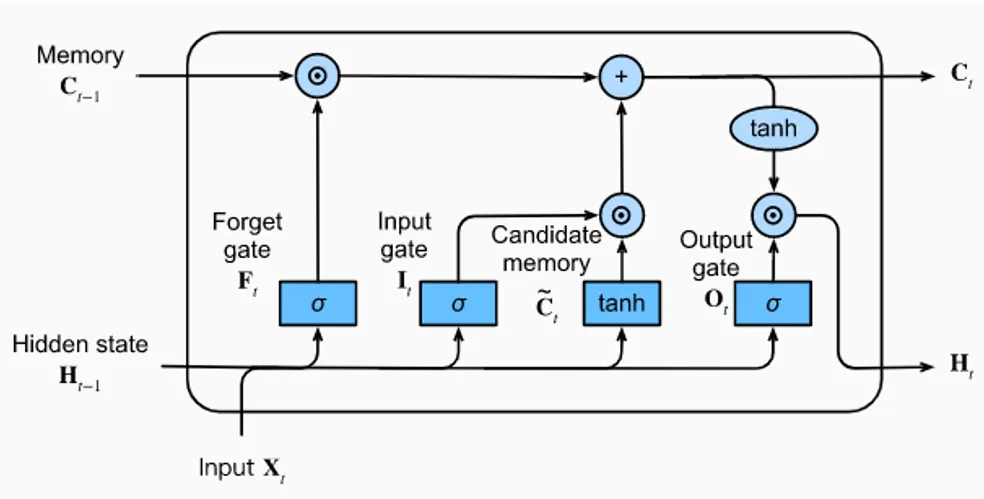
\includegraphics[width=0.75\linewidth]{media/lstm_fig.png}
    \end{center}

    i) The output of the forget gate is defined as 
    $$F_t = \sigma(W_{xf}x_t + W_{hf}h_{t - 1} + b_f)$$
    where $\sigma$ is Sigmoid.
    
    The output of the input gate is defined as 
    $$I_t = \sigma(W_{xi}x_t + W_{hi}h_{t - 1} + b_i)$$
    and is used to select from the candidate memory. The candidate memory is defined as
    $$\tilde{C}_t = \text{tanh}(W_{xc}x_t + W_{hc}h_{t - 1} + b_c)$$
    Then, the updated long-term memory is
    $$C_t = F_t \odot C_{t - 1} + I_t \odot \tilde{C}_t$$
    
    where $\odot$ denotes element-wise multiplication. Explain in 1-2 sentences what the product $I_t \odot \tilde{C}_t$ represents. Explain in 1-2 sentences why it is added to $F_t \odot C_{t - 1}$ to update $C$. \\

    ii) The output of the output gate is defined as
    $$O_t = \sigma(W_{xo}x_t + W_{ho}h_{t - 1} + b_o)$$

    The updated hidden state is 
    $$h_t = O_t \odot \text{tanh}(C_t)$$

    The output for the cell (not shown in the figure) is
    $$\hat{y}_t = \text{softmax}(W_{xh}h_t + b_y)$$

    Explain in 1-2 sentences why we update $h$ by multiplying $O_t$ by $\text{tanh}(C_t)$ element-wise.
    \\

    iii) Implement the \texttt{TODO}s in the \texttt{LSTMLayer} class in \texttt{lstm.py}. Implement the \texttt{TODO}s in the \texttt{LSTM} class in \texttt{lstm.py}. Train the LSTM using \texttt{train\_imbd.py} (look at the \texttt{argparse} for how to switch the model type) for 5 epochs, a minimum sequence length of 0, and a maximum sequence length of 200. Then train the LSTM for 5 epochs, on a minimum sequence length of 200, and a maximum sequence length of 400. Attach your accuracy and loss plots here for both models and report test accuracies.
    
    \end{adjustwidth} 
    \vspace{5px}
\end{adjustwidth}

\end{problem}

\begin{solution*}{}{}
Student solution here.
\end{solution*}